\section{Systeme \skript{109}}
\subsection{Begriffe}
\begin{tabular}{|p{5cm}|p{5cm}|p{7.5cm}|}
\hline & & \\
\textit{Bezeichnung}
	& \textit{Beschreibung}
	& \textit{Bedingung, Erkennung} \\
\hline \hline & & \\
Wirkungsfreiheit \skript{109}
	& Eingang des System hochohmig 
	& Die Eingänge haben keine Rückwirkung auf die Ausgänge der vorhergehenden Systeme.\\
\hline & & \\
Statische bzw. dynamische Systeme \skript{110,111}
	& Ohne(statisch, resistiv) bzw. mit Gedächtnis
	& Statisch: der Ausgang hängt direkt vom Eingang zur Zeit $t_0$ ab.
		$y(t_0) = f(x(t_0))$ $\forall t_0$ \\
	& & Dynamisch: $\int dt; \; \frac{d}{dt}; \; f(t \pm t_0) $\\
\hline & & \\
Kausale bzw. akausale Systeme \skript{112}
	& Keine zukünftigen Werte bzw. nicht in ``Echtzeit''
	& \parbox{7cm}{Kausal: hängt \underline{nicht} von zukünftigen Werten ab.
		$f(t - t_0); \int^t f(\tau) d \tau \quad (t_0 > 0) \quad$ \\ Statische
		Systeme sind immer kausal. \\ \\ 
		Akausal: hängt von zukünftigen Werten ab.
		$f(-t); \; f(t + t_0); \; \int^{t+t_0}
		f(\tau) d \tau$} \\
	\hline & & \\ Zeitinvariante bzw. zeitvariante Systeme  \skript{118} & Von der Zeit (un-) abhängig
	& \parbox{7cm}{
		Zeitvariant: $\cos(t) x(t); t^{\alpha} x(t) \qquad (\alpha \neq 0 )$ \\ \\
		Zeitinvariant: $x(t) \rightarrow y(t)$ , dann gilt\\
		$x(t-t_0) \rightarrow y(t-t_0)$ $\forall t_0$} \\ %$x(t) \rightarrow y(t)$
\hline & & \\
Lineare bzw. nichtlineare Systeme \skript{113}
	&
	& \parbox{7cm}{
			Nichtlinear: $x(t) = 0 \rightarrow y(t) \neq 0 \Rightarrow$\\
			Ausgangssignal, kann Frequenzkomponenten enthalten, welche beim
			Eingangssignal \underline{nicht} enthalten sind.\\ \\ 
			Linear: $S(x1+x2)=S(x1)+S(x2)$ \\ $S(c\cdot x)=c\cdot S(x) \Rightarrow$
			enthält \underline{keine} neuen Frequenzkomponenten im Ausgangssignal.} \\
\hline 
	Reelle Systeme \skript{121} &
	ein reelles Eingangssignal bewirkt immer ein reelles Ausgangssignal& \\
\hline
	Invertierbare Systeme \newline \skript{121} &
	bei jedem Ausgangssignal kann eindeutig auf das Eingangssignal geschlossen werden &
	\parbox{7cm}{
		invertierbar: $y = x^3 \rightarrow x = \sqrt[3]{y}$ \\ \\
		nicht invertierbar: $y=x^2 \rightarrow x = \pm \sqrt{y}$
	}\\
\hline
\end{tabular}

\subsection{Übertragungsfunktion von LTI-Systemen \skript{108}}
\begin{tabular}{ll}
\parbox{10cm}{
	\begin{align}
		h(t) &\; \laplace \; H(s) \nonumber \\
		y(t) = h(t) * f(t) &\; \laplace \; Y(s) = H(s) F(s) \nonumber 
	\end{align}}
	& \parbox{5cm}{
		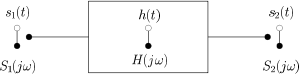
\includegraphics[width=5cm]{./bilder/utf-theorie.png}}\\
$h(t)$: Impulsantwort & $H(s)$: Übertragungsfunktion
\end{tabular} \\

Kaskadierung von wirkungsfreien Systemen:
$H_{total}(s) = H_1(s) H_2(s)$ bzw. bei $n$ gleichen Systemen:
$H_{total} = (H(s))^n$
 \\ \\

\begin{tabular}{ll}
\parbox{13cm}{
	\textbf{Beispiel}: Gesucht UTF $H(s) = \frac{Y(s)}{F(s)}$ \\
	$$H(s) = \frac{sL}{\frac{1}{sC} + sL + R} = \frac{s^2}{\frac{1}{LC} + s
	\frac{R}{L} + s^2}$$\\
	$$\Longrightarrow \text{Pole bei } s = -\frac{R}{2L} \pm j
	\sqrt{\frac{1}{LC} - \left(\frac{R}{2L}\right)^2} \quad ; \quad \text{Doppelte
	Nullstelle bei } s = 0$$
	Differentialgleichung:    $ \ddot{y}(t)+
	\frac{R}{L}\dot{y}(t)+\frac{1}{LC}y=\ddot{x}(t)$}
	
	
	& \parbox{5cm}{
		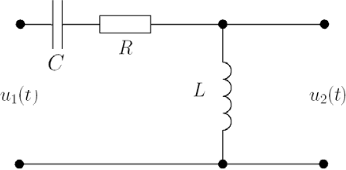
\includegraphics[width=5cm]{./bilder/utf-beispiel.png}} \\
		
\end{tabular}

%\begin{multicols}{2}

\subsubsection{Bestimmung der UTF}
\begin{tabular}{ll}
	Bauteil & Ersatz \\
	R & R\\
	L & sL\\
	C & $\frac{1}{sC}$ \\
\end{tabular}\\
%Parallelschaltung $= \frac{1}{\frac{1}{R}+\frac{1}{sL}+sC}$\\
%Das Potential in einem Punkt berechnet man mit $=\frac{Summe\ aller\
%Elemente\ zwischen\ Punkt\ und\ GND}{Summe\ aller\ Elemente\ der\ Kompletten\
%Schaltung}$\\
%Die Ordnung der UTF ist die Anzahl unabhängiger Speicher (L oder C).\\
%\end{multicols}

\subsection{Berechnung des Amplituden- und Phasengangs aus der
Übertragungsfunktion}
\begin{equation}
	H(j \omega) = \frac{Y(j \omega)}{F(j \omega)} = |H(j\omega)| e^{j\Theta(\omega)} = 
	\frac{|Y(j \omega)|}{|F(j \omega)|} e^{j (\arg(Y(j \omega)) - 
	\arg(F(j\omega)))} =
	\frac{|Y(j \omega)|}{|F(j \omega)|} e^{j \left[\arctan \left(\frac{\Imag\{Y(j
	\omega)\}}{\Real\{Y(j \omega)\}} \right) - \arctan \left(\frac{\Imag\{F(j
	\omega)\}}{\Real\{F(j \omega)\}} \right)\right]} \nonumber \\
\end{equation}


\begin{tabular}{ll}
	Phasengang: & 
	\begin{equation}
		\Theta(\omega) = \arctan \left(\frac{\Imag (H(j\omega))}{\Real (H(j\omega))}\right) \nonumber
	\end{equation} \\
	Amplitudengang: &
	\begin{equation}
		|H(j\omega)| = \frac{|Y(j\omega)|}{|F(j\omega)|} \nonumber
	\end{equation}
\end{tabular}



\subsection{Zusammenhang zwischen Impuls- \& Einheitssprungantwort, Endwerte
\skript{109}}
$ \text{Einheitssprungantwort } g(t) \text{, Impulsantwort }h(t)$
$$h(t)= \frac{\partial g(t)}{\partial t}\quad\text{bzw.}\quad
g(t)=\int_{-\infty}^{t}h(\tau)d\tau \qquad;\qquad 
\lim\limits_{t \rightarrow \infty}  h(t)= \lim\limits_{s \rightarrow 0} s H(s)
\qquad;\qquad
\lim\limits_{t \rightarrow \infty}  g(t)= \lim\limits_{s \rightarrow 0} H(s)$$

\newpage

\subsection{Phasen- \& Gruppenlaufzeit \skript{130}}
\definecolor{gruppe}{rgb}{1,.75,0} % 255,192,0
\definecolor{phase}{rgb}{1,0,0} % 255,0,0
Die \textcolor{phase}{Phasenlaufzeit (phase delay)}  ist nur für reine Sinussignale bestimmbar:
$\tau_P(\omega)=\frac{-\theta(\omega)}{\omega}$ \\
Die \textcolor{brown}{Gruppenlaufzeit (groupe delay)} hingegen ist für sämtliche Signale möglich:
$\tau_G(\omega)=\frac{-\partial\theta(\omega)}{\partial\omega}$\\
Die Signalverzögerung, Phasenlaufzeit $\tau_P(\omega)$ und Gruppenlaufzeit $\tau_G(\omega)$ sind
gleich wenn,
\begin{equation}
	\theta(\omega) = -\omega t_0 \nonumber
\end{equation}
und $H(j\omega)$ die Form $H(j\omega) = a\cdot e^{j\omega t_0}$ hat ($t_0$: Signalverzögerung).\\
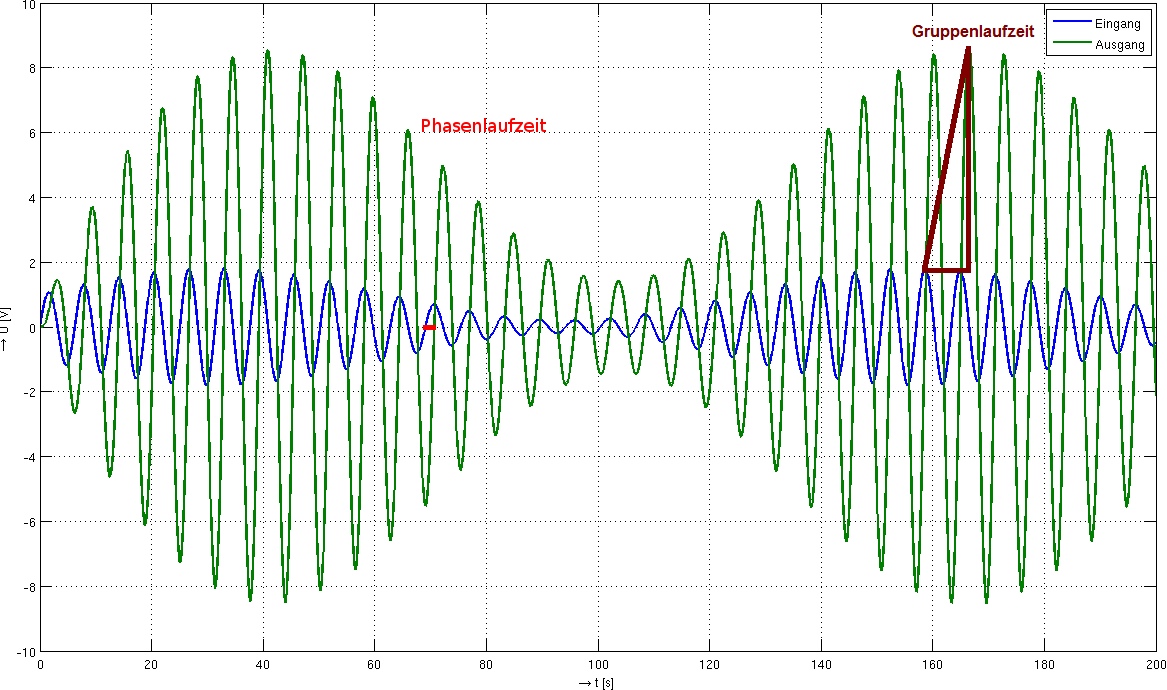
\includegraphics[width=18cm]{./bilder/laufzeit.png}\\
Eingangssignal $x(t)$ und Ausgangssignal $y(t)$ des Systems
$H(s)=\frac{1}{s^2+0.2s+1}$. Bemerkung: $y(t)$ ist gr"osser als $x(t)$.

\subsection{Stabilität von LTI-Systemen \skript{125}}
\subsubsection{BIBO-Stabilität \skript{125}}
	Ein System ist BIBO-stabil (Bounded Input Bounded Output), wenn auf jedes
	beschränkte Eingangssignal das Ausgangssignal ebenfalls beschränkt ist.
	$|u_{in}(t)| < A \rightarrow |u_{out}(t)| < B$ mit $0 < A,B \in \mathbf{N} < \infty$
	\begin{equation}
		\int\limits_{-\infty}^{\infty} |h(t)| dt < \infty \nonumber
	\end{equation}

\subsubsection{Asymptotische Stabilität \skript{126}}
\begin{tabular}{l p{15cm}}
Stabil: 
	& $\lim\limits_{t\rightarrow\infty} h(t) = 0$ 
	\qquad Pole \textbf{nur} in der
linken s-Halbebene.\\
Instabil: 
	& Mind. ein Pol in der rechten s-Halbebene oder mind. ein
\textbf{mehrfacher} Pol auf der $j$-Achse der s-Ebene. \\
Grenzstabil:
	& mindestens ein \textbf{einfacher Pol}, aber \textbf{kein mehrfach Pol} 
		auf der $j$-Achse und \textbf{kein Pol} auf der \textbf{rechten} s-Halbebene
\end{tabular}

\newpage

\subsubsection{Stabilität mit Hurwitz-Polynom \skript{127}}
Es wird jeweils das Polynom im \textbf{Nenner der Übertragungsfunktion} betrachtet:
$P(s) = a_n s^n + a_{n-1} s^{n-1} +\ldots +a_1s + a_0$ \\
Ist ein solches Polynom ein Hurwitz-Polynom, so ist das System \textbf{asymptotisch stabil}.
Handelt es sich um ein \textbf{modifiziertes Hurwitz-Polynom} so ergibt es ein
\textbf{grenzstabiles} System.\\ \\
$P(s)$ ist nur dann ein Hurwitz-Polynom, wenn folgende Bedingungen erfüllt sind:
\begin{enumerate}
	\item	alle Koeffizienten $a_i$ von $P(s)$ sind grösser als Null (und sind vorhanden).\\
				(bis zum und mit Polynomen von Grad 2, ist es notwendig, dass alle Koeffizienten positiv
				sind, damit das Polynom asymptotisch stabil ist)
	\item	alle Hurwitz-Determinanten $D_1$ bis $D_n$ sind grösser als Null\\
				\begin{align}
					D_1 &= a_{n-1} > 0 \nonumber\\
					D_2 &= \left|
						\begin{matrix}
							a_{n-1} & a_n\\
							a_{n-3} & a_{n-2}
						\end{matrix}\right| > 0 \nonumber \\
						&\vdots \nonumber \\
					D_{n-1} &= \left|
						\begin{matrix}
							a_{n-1} & a_n & 0 & 0 & \cdots & 0 \\
							a_{n-3} & a_{n-2} & a_{n-1} & a_n & 0 & 0 \\
							a_{n-5} & a_{n-4} & a_{n-3} & a_{n-2} & \cdots & 0 \\
							\vdots & \vdots & \vdots & \vdots & \ddots & 0 \\
							0 & 0 & 0 & \vdots & 0 & a_1
						\end{matrix}\right| > 0 \nonumber \\
					D_n &= a_0D_{n-1} > 0 \nonumber
				\end{align}
\end{enumerate}

\textbf{Modifiziertes Hurwitz-Polynom}\\
Nebst allen $a_i \geq 0$ müssen alle Hurwitz-Determinanten $D_1, D_2, \ldots, D_{n-2} > 0$
und $D_{n-1} = D_n = 0$ sein. \\ \\

Für Polynome $P(s) = a_n \cdot s^n + a_{n-1} \cdot s^{n-1} + \ldots + a_1 \cdot s^1 + a_0$ vom
Grad n gild für $a_i > 0$:\\
\begin{tabular}{|l||l| l|}\hline
$N$   &   $P(s)$ ist ein Hurwitz-Polynom (stabil) &  $P(s)$ ist ein
modifiziertes Hurwitz-Polynom (grenzstabil) \\ \hline\hline
      1     &      gilt f"ur alle $P(s)$          &  $a_0=0$ \\ \hline
      2     &     gilt f"ur alle $P(s)$           &  $a_1=0$ \\ \hline
      3     &     $a_1a_2>a_0a_3$      &  $a_1a_2=a_0a_3$ \\ \hline
      4     &     $a_3(a_1a_2-a_0a_3)>a_1^2a_4$   &    $a_3(a_1a_2-a_0a_3)=a_1^2a_4$\\ \hline

      5    &     {\footnotesize $a_3a_4>a_2a_5$  und}   &     {\footnotesize $a_3a_4>a_2a_5$} \\
           &     {\footnotesize
           $(a_1a_2-a_0a_3)(a_3a_4-a_2a_5)>(a_1a_4-a_0a_5)^2$}   &  
           {\footnotesize $(a_1a_2-a_0a_3)(a_3a_4-a_2a_5)=(a_1a_4-a_0a_5)^2$} 
           \\ \hline   
\end{tabular}\\
\begin{itemize}
  \item Wenn \textbf{alle Koeffizienten negativ} sind, kann $-1$ ausgeklammert
  werden und in den Zähler verschoben werden\\ $\Rightarrow$ \textbf{System
  stabil} oder \textbf{grenzstabil} (siehe Punkt 3)
  \item Wenn \textbf{ein Koeffizient nicht vorhanden} ist $(a_x = 0)$, dann ist das System
  evtl. grenzstabil, d.h. es ist eine \textbf{Überprüfung mit modifiziertem Hurwitz-Polynom}
  nötig.
\end{itemize}

\newpage

\subsection{Klirrfaktor \skript{137}}
Als Mass für nichtlineare Verzerrungen gilt der \textit{Klirrfaktor}. Betrachtet
wird jeweils der Effektivwert am Ausgang 
$$k = \sqrt{\frac{U_2^2 + U_3^2 + \ldots + U_n^2}{U_1^2 + U_2^2 + \ldots +
U_n^2}} \qquad 0 \leq k \leq 1$$ 
\begin{tabular}{ll}
Teilklirrfaktor (frequenzselektiv) 
	&$k_m =  \frac {U_m} {\sqrt{ U_1^2+ U_2^2 + \ldots + U_n^2} }$ \\
Klirrdämpfungsmass 
	& $a_k = 20 \log \left( \frac1k \right)$ $\qquad$ \\
Teilklirrdämpfungmass 
	& $a_k = 20 \log \left( \frac{1}{k_m} \right)$
\end{tabular}

\subsection{Total Harmonic Distortion (THD) \skript{137}}
$$\text{THD} = \sqrt{ \frac {U_2^2+ U_3^2 + \ldots + U_n^2} {U_1^2} } \qquad
\infty > \text{THD} \geq k \geq 0; \quad \text{Für kleine Verzerrungen: THD}
\approx k $$

\subsection{Verzerrungsfreie Übertragung von Signalen \skript{138}}
	Bedingungen für eine verzerrungsfreie Übertragung:\\
	\begin{tabular}{lll}
		1. & Amplitude: & konstant (unabhängig von der Frequenz) $\leftrightarrow
			|H(j\omega)| = \text{konstant} = a \neq 0$ \\
		2. & Phase: & proportional zur Frequenz $\leftrightarrow
			\Theta(\omega) = -\omega t_0$ 
	\end{tabular}
	
\subsection{Übertragung von stochastischen Signalen \skript{141}}
\begin{tabular}{|l|l|}
	\hline
		lineare Mittelwert $Y_0$: &
		$Y(j0) = X(j0) \cdot H(j0) \rightarrow Y_0 = X_0 \cdot H(j0)$ \\
	\hline
		Autokorrelation: &
		$\varphi_{yy}(\tau) = \int\limits_{-\infty}^{\infty} \int\limits_{-\infty}^{\infty}
		h(\alpha)h(\beta)\varphi_{xx}(\tau+\alpha-\beta)d\alpha d\beta = h(-\tau) * h(\tau) * \varphi_{xx}(\tau)$\\
		& $\varphi_{yy}(\tau) = \frac{1}{2\pi} \int\limits_{-\infty}^{\infty}|H(j\omega)|^2 \phi_{xx}(j\omega)
		e^{j\omega \tau} d\omega$ \\
	\hline
		Leistungsdichtespektrum: &
		$\phi_{yy}(j\omega) = |H(j\omega)|^2\phi_{xx}(j\omega)$\\
	\hline
		Leistung: &
		$Y^2 = \varphi_{yy}(0) = \frac{1}{2\pi}\int\limits_{-\infty}^{\infty}|H(j\omega)|^2\phi_{xx}(j\omega) d\omega$\\
	\hline
		Kreuzkorrelation: &
		$\varphi_{xy}(\tau) = h(\tau) * \varphi_{xx}(\tau) \; \laplace \; \phi_{xy} = H(j\omega) \cdot \phi_{xx}(j\omega)$ \\
		& $\varphi_{yx}(\tau) = h(-\tau) * \varphi_{xx}(\tau) \; \laplace \; \phi_{yx} = H^*(j\omega) \cdot \phi_{xx}(j\omega)$ \\
		& $\varphi_{yx}(\tau) = \varphi_{xy}(-\tau) \; \laplace \; \phi_{yx}(j\omega) = \phi_{xy}(-j\omega) = \phi_{xy}^*(j\omega)$\\
	\hline
\end{tabular}